\chapter{Einleitung}\label{chap:introduction}

\section{Über die Arbeit}

Diese Arbeit beschreibt die Konzipierung und Entwicklung einer Anwendung, die es ermöglichen soll, erkrankte Nutzpflanzen wie angebautes Getreide und Gemüse früh zu identifizieren. Des Weiteren wird die Performanz der Anwendung überprüft und anschließend die Ergebnisse präsentiert.
\\\\
Dieses Kapitel gibt einen kurzen Überblick über die Arbeit. Es wird erläutert, welche Auswirkungen Krankheiten auf die Agrarwirtschaft haben und infolgedessen, wie sich die Motivation der Thematik daraus bildet.
\\\\
Kapitel 2 geht auf die Herkunft der Realdaten ein und beschreibt wie Satellitendaten über Felder gewonnen und verarbeitet werden können. Es werden Anforderungen an ein künstliches neuronales Netzwerk festgelegt und erörtert, warum das dort beschriebene Netzwerk ausgesucht wurde. Anschließend wird eine Methode definiert, um die späteren Ergebnisse zu evaluieren.
\\\\
Overfitting ist eine bekannte Herausforderung im Bereich des maschinellen Lernens. Daher wird in Kapitel 3 erklärt, was Overfitting ist und wie man dem entgegenwirken kann.
\\\\
Kapitel 4 beschreibt die Konzipierung der Prozessschritte der Anwendung und erläutert Implementationdetails. Die manuelle Annotation der Trainingsdaten, die Aufbereitung der Satellitendaten und das Training des neuronalen Netzwerks werden aufgezeigt. Ebenfalls wird die Konfiguration des Netzwerkes erklärt.
\\\\
In Kapitel 5 werden einige Experimente erklärt, die auf Basis der in Kapitel 3 gezeigten Methoden definiert wurden. Zusätzlich werden die Ergebnisse der Experimente diskutiert und Erkenntnisse formuliert, die daraus gewonnen wurden.
\\\\
Das sechste Kapitel fasst die Arbeit zusammen und zieht ein Fazit aus den Ergebnissen. Zuletzt schließt ein kurzen Ausblick die Arbeit ab.

\section{Motivation}

Krankheitserreger sorgen für hohe Ertragsverluste und verursachen dadurch große wirtschaftliche Schäden und erschwert die Nahrungsproduktion für die immer weiter wachsende Weltbevölkerung. Die globalen Ernteeinbußen durch Krankheiten und Schädlinge werden auf etwa 30\% geschätzt.\cite{ref:spiegel} Zum Beispiel ist Sorghumhirse die fünft-wichtigste Getreideart in der Welt. Jedoch können allein Befälle von Sorghum-Antraknose, ein durch Pilzbefall verursachtes Pathogen, einen Ertragsausfall von bis zu 50\% erwirken.\cite[S. 77]{ref:zeller}
\\\\
\begin{figure}[ht]
  \centering
  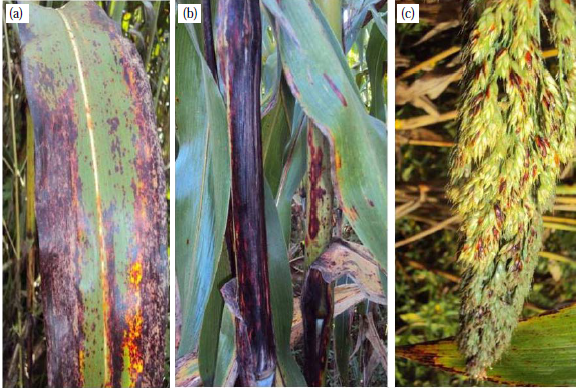
\includegraphics[width=.7\textwidth]{pics/anthracnose.PNG}
  \caption[Sorghum-Anthraknose]{Sorghum-Anthraknose\cite[S. 77]{ref:tsedaley}}
  \label{fig:anthracnose-infected}
\end{figure}
\noindent
Pestizide und andere Chemikalien ermöglichen die Bekämpfung von Befällen. Jedoch hat ein exzessiver Einsatz von Pestiziden einen negativen Effekt auf die Umwelt. So sickert es in den Ackerboden und kann das Grundwasser kontaminieren. Daher ist es wichtig, dass Landwirte regelmäßig ihre Felder auf mögliche Schäden untersuchen und diese gezielt eindämmen. Da Landwirte in der Regel großflächige Gebiete betreiben, stellt sich eine manuelle Kontrolle als schwierig dar. Zumal sichtbare Symptome schon Zeichen für einen schweren Befall sein können.
\\\\
Bemannte oder unbemannte Fluggeräte können die Überwachung unterstützen und schnelle Einschätzungen über den aktuellen Gesundheitsstatus der Äcker geben. So untersuchten Pugh et al. die Fähigkeit einer unbemannten Flugdrohne Anthraknosebefälle in Sorghumfelder einzuschätzen. Sie kamen zu dem Schluss, dass die Methode effektive Analysen zurückgeben kann und durch die Flugeigenschaft eine größere Reichweite hat als traditionelle Fern-überwachungssysteme.\cite[S. 861ff.]{ref:pug}
\\\\
\begin{figure}[ht]
  \centering
  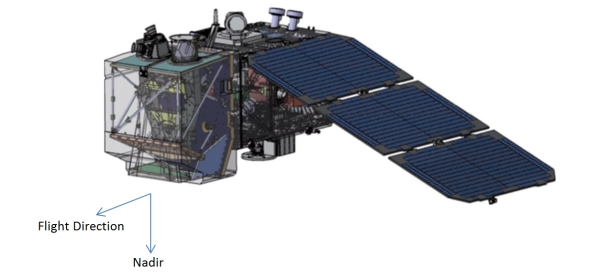
\includegraphics[width=.7\textwidth]{pics/sentinel.jpg}
  \caption[Schematische Ansicht Sentinel-2]{Schematische Ansicht Sentinel-2\cite{ref:sentinel:descr}}
  \label{fig:anthracnose}
\end{figure}
\noindent
Fluggeräte sind jedoch dadurch eingeschränkt, dass sie nur so lange fliegen können, wie es ihr Energiefüllstand (Kerosin bei Flugzeugen, Batterieladestand bei kleinen Drohnen, \dots) zulässt. Das heißt, dass sie mit Treibstoff versorgt werden müssen, der die Landwirte auch weiter monetär belastet. Raumfahrende Überwachungsinstrumente wie Satelliten, die die Erde in einem hohen Orbit umkreisen, liefern regelmäßige Aufnahmen von nahezu jedem Punkt der Erde. So kann man auf die Aufnahmen der Sentinel-Satelliten des Copernicus-Programms zugreifen und zur eigenen Feldüberwachung nutzen. Chemura, Mutange und Dube zeigten, dass man über Multispektralaufnahmen der Sentinel-2-Plattform unter Laborbedingungen die Schwere einer Kaffeerosterkrankung einschätzen kann.\cite[S. 877]{ref:chemura} Dennoch wird erwähnt, dass Feldtesttauglichkeit noch getestet werden muss.\cite[S. 859]{ref:chemura} Diese Arbeit greift diese Idee auf, nutzt dabei aber nicht die Methoden aus dem Paper. Zum einem, da Nutzpflanzen untersucht werden sollen, die anders als Kaffee im europäischen Raum angebaut werden. Und zum anderen ist ein Ziel dieser Arbeit, ein infiziertes Feld möglichst genau eingrenzen zu können. 